% !TeX root = ./Main.tex
% !TeX engine = xetex
% !BIB program = bibtex

\documentclass[oneside, openbib, parskip = full-]{scrartcl}
% \includeonly{ % #INFO: wenn man nur bestimmte includes nutzen will
%     content/Anhang_KIS
%     }

\def\myStudentenname{Marco von Rosenberg}
\def\myTitle{Spatio-Temporal Predictions am Beispiel von Geschwindigkeitskontrollen}
\def\myDokumententyp{Studienarbeit}
%\def\myBachelorart{Bachelor of Science (B.Sc.)} % aus kommentieren wenn keine Bachelorarbeit
\def\myStudiengang{Informatik/Informationstechnik}
\def\myHochschule{Dualen Hochschule Baden-Württemberg Stuttgart}
\def\myMatrikelnummer{9594981}
\def\myKurs{TINF19IN}
\def\myAusbildungsfirma{Keysight Technologies, Böblingen}
\def\myErstgutachter{Johannes Staib}
%\def\myZweigutachter{Vorname Nachname} % aus kommentieren wenn es keinen gibt
\def\myTitleHeaderImage{content/images/DHBW_Logo.png}
\def\myOrt{Stuttgart}
\def\Bearbeitungszeitraum{13. September 2021 - \today} % Bearbeitungszeitraum % #INFO: allgemeine Werte für die Arbeit

%%%
%%% KOMA related
%%%

\usepackage[
    paper=a4paper,
    left=25mm,
    right=25mm,
    top=25mm,
    bottom=20mm,
    includefoot,
    foot=\baselineskip,
    bindingoffset=0mm
]{geometry}

\usepackage[utf8]{inputenc} % encoding
\usepackage[T1]{fontenc} % selecting font encodings
\usepackage[ngerman]{babel} % German hyphenation
\usepackage[babel,german=quotes]{csquotes} % German quotes
\usepackage{lmodern} %MOST IMPORTANT PACKAGE!!! High resolution font
\renewcommand*\familydefault{\sfdefault} %% für Serifen freie Schrift
\usepackage{textcomp} % für in line {\textmu}

\usepackage{scrlayer-scrpage}
\clearpairofpagestyles
\setkomafont{pageheadfoot}{\sffamily\footnotesize}
\setkomafont{pagehead}{\bfseries}
\setkomafont{pagination}{}

\KOMAoptions{
    headsepline = true,
    footsepline = false,
    plainfootsepline = false
}
\renewcommand*{\sectionmarkformat}{}

\automark{section}
\ihead{\myStudentenname}
\chead{\myDokumententyp}
\ohead{\headmark}
\ofoot*{\pagemark}


\usepackage{scrdate} % Für Datum und Wochentag

%%%
%%% not KOMA related
%%%


\usepackage[onehalfspacing]{setspace}

%\usepackage{booktabs} %Never, ever use vertical rules! Never use double rules!
\usepackage{multirow}
\usepackage{comment}

%\usepackage{etoolbox} %use with care! powerful but not can create difficult errors! extends build time
%\AtBeginEnvironment{table}{\sffamily}
%\AtBeginEnvironment{tabular}{\sffamily}

%\usepackage{enumitem}
\usepackage{paralist} % for \begin{compactitem}

% Much much better listings
\usepackage[newfloat, outputdir=aux]{minted}
\newenvironment{code}{\captionsetup{type=listing}}{}
\SetupFloatingEnvironment{listing}{name=Codeausschnitt}

\usepackage{listings}
\lstset{
    basicstyle=\footnotesize, % Global Code Style
    numbers=left,
    numberstyle=\tiny,
    columns=flexible,
    breaklines=true,
    postbreak=\mbox{\textcolor{red}{$\hookrightarrow$}\space},
}
% from https://tex.stackexchange.com/questions/303465/higher-asterisks-in-lstlisting-environment
\makeatletter
\lst@CCPutMacro
    \lst@ProcessOther {"2A}{\raisebox{2pt}{*}}
    \@empty\z@\@empty
\makeatother

\usepackage{etex}
% \#TODO: Entscheiden welchen Style
\bibliographystyle{myIEEEtran}
%\bibliographystyle{ieeetr} % ist ohne den Strich
%\bibliographystyle{IEEETran} % ist mit dem Strich, dafür ausführlicher


\usepackage{graphicx}
%\usepackage{svg} %no reason to use this (unless you know how to use it)
\usepackage{float}
\usepackage[abs]{overpic} % Für Unterschrift

\usepackage[binary-units = true ]{siunitx}
%\sisetup{scientific-notation = true} % Wissenschaftliche Notation
\sisetup{exponent-product = \cdot}
\sisetup{output-product = \cdot} % Das Punkt statt X
\sisetup{binary-units=true}
\sisetup{output-decimal-marker = {,}}
\sisetup{detect-all} 	% Einstellung das Front für SI gleich Standardfront
\sisetup{per-mode = symbol}
\sisetup{locale=DE}
\usepackage{eurosym}
\DeclareSIUnit{\sieuro}{\mbox{\euro}}

% verwende gerade kein Mathe \usepackage{amsmath, amsthm, amssymb}
% !sehr langsam  \usepackage[colorinlistoftodos,prependcaption, textsize=footnotesize]{todonotes}
\usepackage{amsmath, amssymb}


%\usepackage{booktabs}
\usepackage{graphicx}
\usepackage{adjustbox}
\usepackage{subcaption}
%\usepackage{lscape}
%\usepackage{tikz}
\usepackage{pgfplots}
\pgfplotsset{compat=1.16}
\usepackage{pgfplotstable}

%% Glossar
\usepackage[acronym,nonumberlist,nopostdot]{glossaries}
\newcommand\acrfullr[2][]{\acrshort[#1]{#2} (\acrlong[#1]{#2})}
\usepackage{glossary-mcols} % für Style mcolindex
\glsenablehyper % Verlinkung der Einträge im Text zu Abkürzungen
\setglossarystyle{mcolindex}
\renewcommand{\glossarypreamble}{\glsfindwidesttoplevelname[\currentglossary]} % funktioniert nicht mit mcolindex
\makenoidxglossaries


\usepackage{makecell} % Für multiline Zellen mit \makecell
%\usepackage{tabularx}
\usepackage{longtable}


\usepackage[
    hidelinks,              % Das Links nicht farbig
    bookmarks,              % Bookmarks erstellen
    bookmarksopen,          % Bookmarks bei öffnen des PDF anzeigen
    bookmarksnumbered,      % damit Nummern in Bookmarks
    bookmarksopenlevel = 1, % damit nur die erste Ebene der Bookmarks beim öffnen angezeigt werden
    pdftoolbar=		false,
    pdfmenubar=		false,
    pdftitle={		\myDokumententyp~über~\myTitle~von~\myStudentenname},
    pdfsubject={}
    pdfkeywords={}
    pdfauthor={		\myStudentenname},
    pdfstartpage={	1}
    ]{hyperref}
\addto\extrasngerman{\def\subsectionautorefname{Abschnitt}}
\addto\extrasngerman{\def\subsubsectionautorefname{Abschnitt}}
\addto\extrasngerman{\def\appendixautorefname{Anhang}} % funktioniert auch nicht
\addto\extrasngerman{\def\lstlistingautorefname{Codeausschnitt}}
\renewcommand{\lstlistingname}{Codeausschnitt}

%% Anhang
\usepackage{appendix}
\renewcommand{\appendixname}{Anhang}
\renewcommand{\appendixtocname}{Anhang}
\renewcommand{\appendixpagename}{Anhang}
%\newcommand{\appendixautorefname}{Anhang} % funktioniert nicht
\newcommand*\appendixmore{% see the KOMA-Script documentation
\clearpage
%\addsec{{\appendixname}}%
\renewcommand{\thesubsection}{{\Alph{subsection}}}%
} % damit Appendix subsection mit Buchstaben anfangen

\newcommand{\appendixref}[1]{\hyperref[#1]{Anhang~\ref{#1}}}

\renewcommand{\k}[1]{\textit{#1}}
\newcommand{\f}[1]{\textbf{#1}}
\let\oldautoref\autoref
\let\oldref\ref

\renewcommand{\autoref}[1]{\oldautoref{#1}}
\renewcommand{\ref}[1]{\oldref{#1}}
\newcommand{\fullref}[1]{\autoref{#1} \nameref{#1}}  % #INFO: Einstellungen
%\newglossaryentry{control endpoint}{name={control endpoint}, description={logische, addressierte Schnittselle in \acrshort{usb} }}
%\newglossaryentry{ieee488}{name={IEEE-488},description={}}

% Abkürzungen
\newacronym{nn}{NN}{\k{neuronales Netz}}
\newacronym{relu}{ReLU}{\k{rectified linear unit}}
\newacronym{mse}{MSE}{\k{mean squared error}}
\newacronym{rnn}{RNN}{\k{rekurrentes neuronales Netz}}
\newacronym{lstm}{LSTM}{\k{Long Short Term Memory}}
\newacronym{cnn}{CNN}{\k{convolutional neural network}}
\newacronym{rgb}{RGB}{\k{Rot Grün Blau}}
 % #INFO: laden aller Glossary und Abkürzungen

\begin{document}
%%%
%%% Vorbau
%%%
\pagenumbering{Roman}
\begin{titlepage}
	\thispagestyle{empty}
    \begin{center}
        \scalebox{0.6}{\includegraphics[width=\textwidth]{\myTitleHeaderImage}}
        \vspace{1cm}
        \\
        \rule{\textwidth}{1.6pt}\vspace*{-\baselineskip}\vspace*{2pt}
        \rule{\textwidth}{0.4pt}
        \\[0.2\baselineskip]
        {\LARGE \myTitle}
        \rule{\textwidth}{0.4pt}\vspace*{-\baselineskip}\vspace{3.2pt}
        \rule{\textwidth}{1.6pt}
        \\
        \vspace*{12mm}	{\large \myDokumententyp}\\
        \ifx\myBachelorart\undefinde
            \vspace*{27mm}	des Studiengangs \myStudiengang\\
        \else
            \vspace*{12mm}	für die Prüfung zum\\
            \vspace*{3mm} 	{\large \myBachelorart}\\
            \vspace*{12mm}	Studienganges \myStudiengang\\
        \fi
        \vspace*{3mm} 	an der \myHochschule\\
        \vspace*{12mm}	von\\
        \vspace*{3mm} 	{\large \myStudentenname}\\
        \vspace*{12mm}	{\todaysname}, der {\today} \\
      \end{center}

      \vfill
      \begin{spacing}{1.2}
        \centering
        \begin{tabbing}
            \hspace{6.5cm}                   \= \kill\\
            \textbf{Matrikelnummer, Kurs}  \>  \myMatrikelnummer, \myKurs\\
            \textbf{Ausbildungsfirma}      \>  \myAusbildungsfirma\\
            \textbf{Betreuer}         \>  \myErstgutachter\\
            \ifx\myZweigutachter\undefined
            \else
            \textbf{Zweitgutachter}        \>  \myZweigutachter\\
            \fi
            \textbf{Bearbeitungszeitraum}  \>  \Bearbeitungszeitraum\\
        \end{tabbing}
      \end{spacing}
\end{titlepage}
\section*{Selbständigkeitserklärung}
\vspace{1cm}
\begin{tabbing}
    \hspace{.175\textwidth} \= \hspace{.825\textwidth}\=\kill\\
    Name:		            \> \myStudentenname\\
    Matrikelnummer:		    \> \myMatrikelnummer\\
    Studiengang:		    \> \myStudiengang\\
    Kurs:				    \> \myKurs\\
    Titel:	                \> \myTitle             \>\\
\end{tabbing}
\vspace{1cm}
Ich versichere hiermit, dass ich die vorliegende Arbeit selbstständig verfasst und
keine anderen als die angegebenen Quellen und Hilfsmittel benutzt habe.\\
Falls sowohl eine gedruckte als auch elektronische Fassung abgegeben wurde,
versichere ich zudem, dass die eingereichte elektronische Fassung mit der gedruckten
Fassung übereinstimmt.\\
\vspace{2cm}\\

\begin{figure}[h]
    \centering
    
\includegraphics[width=0.8\textwidth,height=10cm,keepaspectratio=true]{content/images/unterschrift.jpg}
\end{figure}
\vspace{-0.4cm}
\begin{minipage}{0.99\textwidth}
	\centering
	\begin{minipage}[t]{0.5\textwidth}
	\hspace{1cm}
		\begin{tabular}{@{}l@{}}\hline
			\makebox[7cm]{Ort, Datum}\\
			\\
			\\
		\end{tabular}
	\end{minipage}
	\hfill
	\begin{minipage}[t]{0.4\textwidth}
		\begin{tabular}{@{}l@{}}\hline
			\makebox[5cm]{Unterschrift}\\
			\\
			\\
		\end{tabular}
	\end{minipage}
\end{minipage}

\section*{Abstract}
\#TODO: Abstract
\section*{Kurzfassung}
\#TODO: Kurzfassung

% --- Inhaltsverzeichnis ---
\pdfbookmark[section]{\contentsname}{toc}
\tableofcontents

\clearpage
% --- Abbildungsverzeichnis --
\phantomsection
\addcontentsline{toc}{subsection}{Abbildungsverzeichnis}
\listoffigures

% --- Tabellenverzeichnis ---
\phantomsection
\addcontentsline{toc}{subsection}{Tabellenverzeichnis}
\listoftables

% --- Listing Verzeichnis --- % #INFO: Verwende ich gerade nicht
\phantomsection
\addcontentsline{toc}{subsection}{Codeausschnittsverzeichnis}
\lstlistoflistings

% --- Glossar ---
\iffalse % #INFO: auf \iftrue setzen falls man ein Glossar will
\phantomsection
\addcontentsline{toc}{subsection}{Glossar}
\printnoidxglossary[sort=word,title=Glossar] % main glossary
\fi

% --- Abkürzungen ---
\phantomsection
\addcontentsline{toc}{subsection}{Abkürzungen}
\printnoidxglossary[type=acronym,title=Abkürzungen] % Abkürzungen


\clearpage

%%%
%%% Inhalt
%%%
\pagenumbering{arabic}
% #INFO: für Inhalt normalerweise \input. \include with care, kann Verweise und so schwieriger machen
% ich nutze trotzdem include damit ich mit \includeonly{} zum test bauen kleiner PDFs erstellen lassen kann
%\input{content/<Name des Kapitels>}
%\include{content/<filename>}

\section{Einführung}
\label{sec:Einführung}

\subsection{Problemstellung und Zielsetzung}
\label{sec:Problemstellung}
In der App \emph{Blitzer.de} können Benutzer mobile und teilstationäre Radarkontrollen sowie Staus, Unfälle und sonstige Gefahren melden.
Diese werden anderen Benutzern angezeigt, wodurch sie vorgewarnt sind und sich entsprechend vorsichtig verhalten können.
Jedoch sind die Meldungen naturgemäß zeitverzögert, da aktive Benutzer benötigt werden, um sie aktuell zu halten.
Es lässt sich argumentieren, dass die Zeitverzögerung insbesonders in den frühen Morgenstunden und in ländlichen Gebieten signifikant ist,
da sich hier nur wenige Benutzer auf den Straßen befinden.
Dies ist besonders für mobile Radarkontrollen entscheidend, da solche jeden Tag zu unterschiedlichen Zeiten und an unterschiedlichen Orten auf- und abgebaut werden.

Andererseits ist auch denkbar, dass es Zusammenhänge zwischen vergangenen und zukünftigen Standorten von Radarkontrollen gibt.
Dies ist, wie Chollet in \cite{DeepLearningPythonKeras} auf Seite 152 argumentiert, eine wichtige Annahme, derer man sich bei jeglichen Vorhersagen bewusst sein muss.
Diese Zusammenhänge haben im vorliegenden Anwendungsfall sowohl räumliche als auch zeitliche Aspekte.
Beispielsweise liegt es nahe, dass mobile Radarkontrollen zeitlich möglichst gut gestreut werden.
Daher kann man annehmen, dass die Gefahr für eine mobile Radarkontrolle an einem Ort eher gering ist, wenn dort am vorherigen Tag eine solche anzutreffen war.
Die Gefahr sollte jedoch stetig steigen, je länger an diesem Ort keine Radarkontrolle steht.
Eine beispielhafte Annahme für ein rein räumlicher Zusammenhang ist, dass mobile Radarkontrollen in ländlichen Gebieten selten sehr dicht aufeinander folgen.
Befindet sich also an einem bestimmten Ort eine mobile Radarkontrolle, ist es unwahrscheinlich, in direkter Umgebung eine weitere Radarkontrolle anzutreffen.
Je weiter weg man sich begibt, desto weiter steigt die Wahrscheinlichkeit jedoch.

Das Ziel der vorliegenden Arbeit ist daher, die Gefahr für mobile Radarkontrollen anhand historischer Daten und insbesondere derer der letzten Tage für den Folgetag zu prognostizieren.
Wie in \autoref{sec:VerwandteForschung} gezeigt wird, gibt es einige vielversprechende Ansätze, wie Neuronale Netze (\Acrshortpl{nn}) verwendet werden können, um sehr ähnliche Problemstellungen anzugehen.
Ähnliche Problemstellungen sind in diesem Fall Vorhersagen mit räumlichen und zeitlichen Aspekten, wie z.B. die Vorhersage von Verkehrsunfällen oder Verbrechen.
Daher sollen auch in dieser Arbeit \Acrshortpl{nn} verwendet werden, um die Vorhersagen anzustellen.

Die erwähnten historischen Daten bestehen aus allen gemeldeten Standorten von mobilen Radarkontrollen der vorhergegangenen Jahre.
Dieser Datensatz wurde freundlicherweise von der Eifrig Media GmbH bereitgestellt.
Die Eifrig Media GmbH steht hinter der Entwicklung der oben genanten App \emph{Blitzer.de}.
Der Datensatz enthält über 7,7 Millionen gemeldete mobile Radarkontrollen vom 22.05.2014 bis zum 25.10.2021.
Daraus ergibt sich ein Zeitraum von 2713 Tagen und somit ca. 21.300 Meldungen pro Tag.
Die Meldungen beschränken sich hierbei auf Deutschland, wobei die Eifrig Media GmbH in \cite{AboutBlitzerDe} angibt, auch äquivalente Angebote zu \emph{Blitzer.de} im Ausland bereitzustellen.
Jeder Eintrag des Datensatzes enthält u.A. die Koordinaten, sowie den ungefähren Aufbau- und Abbauzeitpunkt der Radarkontrolle.
Diese Daten basieren jedoch auf den Angaben der Appbenutzer und sollten daher nicht unkritisch betrachtet werden.
So entsprechen die Koordinaten dem Standort des Appbenutzers zum Zeitpunkt der Meldung in der App.
Da die Meldungen meist bei laufender Fahrt erfolgen, kann die gemeldete Position auf einem Straßenabschnitt relativ weit vor oder nach der tatsächlichen Position der Radarkontrolle liegen.
Der Abbauzeitpunkt basiert ebenfalls auf Angaben der Appbenutzer.
Sobald ein Benutzer an einer eingetragenen Radarkontrolle vorbeigefahren ist wird dieser gefragt, ob die Radarkontrolle gesehen wurde.
Sobald genügend Benutzer dies verneint haben wird die Radarkontrolle anderen Benutzern nicht mehr angezeigt.
Dieser Zeitpunkt entspricht dann auch dem Abbauzeitpunkt.
Da prinzipiell auch Fehlmeldungen möglich sind, ist es wichtig, die Gesamtdauer der Meldung zu betrachten.
Beträgt die Gesamtdauer beispielsweise nur 10 Minuten kann davon ausgegangen werden, dass es sich um eine Fehlmeldung handelt.
Je länger die Gesamtdauer hingegen ist, desto höher ist die Wahrscheinlichkeit, dass es sich um eine valide Meldung handelt, die von vielen Benutzern bestätigt wurde.

Sowohl die Ungenauigkeit der gemeldeten Position als auch die Möglichkeit für Fehlmeldungen machen es erforderlich, den Datensatz aufzubereiten.
Es bietet sich an, den betrachteten Bereich in ein Raster zu unterteilen und jede Meldung am betrachteten Tag derjenigen Rasterzelle zuzuordnen, in deren Bereich die Meldung liegt.
Dieses Vorgehen macht die Ungenauigkeit der Position sowie die Ungenauigkeit des Auf- und Abbauzeitpunkts weniger signifikant.
Die genaue Vorgehensweise bei der Aufbereitung des Datensatzes wird in \autoref{sec:Datensatz} erläutert.

\subsection{Aufbau der Arbeit}
\label{sec:Aufbau}
%TODO: Überhaupt nötig oder einfach weglassen?



\section{Grundlagen}
\label{sec:Grundlagen}

In diesem Abschnitt werden die Grundlagen des Deep Learning und zweier häufig verwendeter Modelle erläutert.
Dies dient einer schrittweisen Heranführung an das letztendlich verwendete Modell.

\subsection{Deep Learning}
\label{sec:DeepLearning}


\subsection{Long Short Term Memory}
\label{sec:LSTM}

Die einzige bisher vorgestellte Architektur von \acrshortpl{nn} ist das Feedforward-Netz.
Diese Netzarchitektur eignet sich gut für Klassifizierungsaufgaben.
Die vorliegende Arbeit beschäftigt sich jedoch mit Standorten von mobilen Radarkontrollen über die Zeit, also mit sequenziellen Daten.
Feedforward-Netze können zeitliche Zusammenhänge nicht darstellen und nicht erlernen, da sie keinen internen Zustand haben.
Das bedeutet, dass die Ausgabe des \acrshort{nn}s nur abhängig von der aktuellen Eingabe ist, nicht aber von vorherigen Eingaben.

Abhilfe hierbei bieten \k{rekurrente neuronale Netze} (\acrshortpl{rnn}).
Wie Chollet in \cite[S. 252]{DeepLearningPythonKeras} erläutert, besitzen rekurrente \acrshortpl{nn} einen internen Zustand, der alle bisherigen Eingaben repräsentiert.
Eine Ausgabe ist dann sowohl von der Eingabe als auch vom internen Zustand abhängig.
Implementiert wird dieses Verhalten durch eine Schleife im \acrshort{nn}.
In \autoref{fig:RNNSchleife} ist diese Architektur schematisch dargestellt.

\begin{figure}[h]
    \centering
    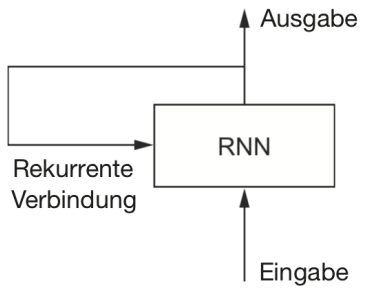
\includegraphics[width=0.5\textwidth,height=4cm,keepaspectratio=true]{content/images/RNNSchleife.png}
    \caption{Schleife in einem \acrshort{rnn} \cite[Abb. 6.9]{DeepLearningPythonKeras}}
    \label{fig:RNNSchleife}
\end{figure}

Ein einfaches \acrshort{rnn} berechnet die Ausgabe $Y_t$ nach \cite[S. 253]{DeepLearningPythonKeras} wie in \autoref{eq:RNN} gezeigt.

\begin{equation}
    Y_t = a(W \cdot X_t + U \cdot S_t + b)
\label{eq:RNN}
\end{equation}

Dabei steht $X_t$ für die Eingabe und $S_t$ für den internen Zustand, jeweils zum Zeitschritt $t$.
$W$ und $U$ sind Matrizen, die die trainierbaren Gewichtungen enthalten und $b$ ist ein trainierbarer Bias-Vektor.
Nach der Berechnung wird die Ausgabe zum neuen internen Zustand, man könnte also $S_t$ in \autoref{eq:RNN} durch $Y_{t-1}$ ersetzen.

Diese einfache Architektur unterliegt nach \cite[S. 260]{DeepLearningPythonKeras} jedoch dem sogenannten \emph{Problem des verschwindenden Gradienten}.
Dieser Effekt sorgt dafür, dass relativ weit zurückliegende Eingaben praktisch keinen Einfluss mehr auf die Ausgabe haben.
Es sind jedoch Anwendungsfälle denkbar, in denen auch weiter zurückliegende Ereignisse einen großen Einfluss auf die Gegenwart haben.
Für die Vorhersage von mobilen Radarkontrollen könnte beispielsweise von Bedeutung sein, wie die Verteilung der Radarkontrollen vor 15 Tagen ausgesehen hat.
Das liegt daran, dass die Daten eine Periodizität von z.B. 15 Tagen aufweisen könnten.

Zur Lösung dieses Problems gibt es verschiedene alternative \acrshort{rnn}-Architekturen.
Eine davon ist \acrfull{lstm}.
Wie der Name vermuten lässt, ermöglicht die \acrshort{lstm}-Architektur, sowohl Abhängigkeiten von weit zurückliegenden als auch aktuellere Eingaben zu lernen.
Die \acrshort{lstm}-Architektur ist in \autoref{fig:LSTMCell} dargestellt.

\begin{figure}[h]
    \centering
    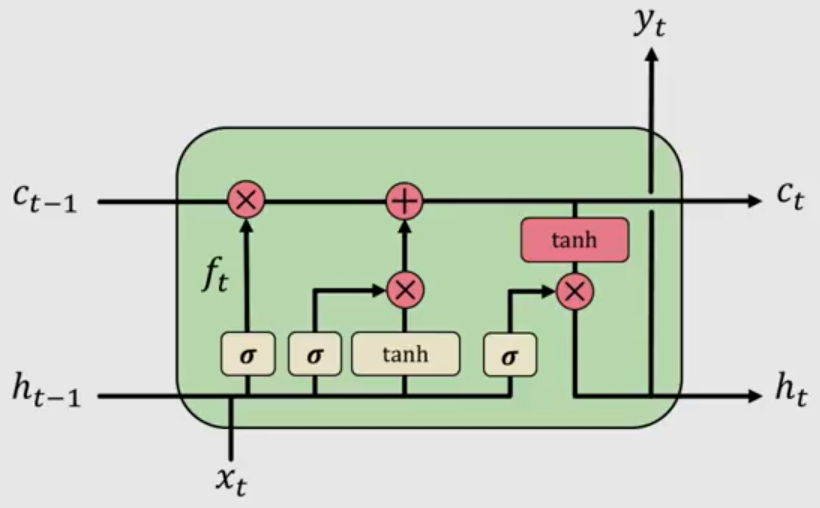
\includegraphics[width=0.8\textwidth,height=6cm,keepaspectratio=true]{content/images/LSTMCell.png}
    \caption{Schematische Darstellung einer \acrshort{lstm}-Zelle \cite{6S191RNN}}
    \label{fig:LSTMCell}
\end{figure}

Eine \acrshort{lstm}-Zelle enthält drei sogenannte Tore (engl. Gates).
Ein Tor ist selbst ein \acrshort{nn}.
Die drei Tore und ihre jeweilige vorgesehene Wirkung sind nach \cite{6S191RNN}:

\begin{enumerate}
    \setlength\itemsep{0.2em}
    \item \textbf{Vergessens-Tor}: Dieses Tor sorgt dafür, dass irrelevante Informationen aus dem vorherigen Zustand "`vergessen"' werden.
    \item \textbf{Merk-Tor}: Dieses Tor fügt dem Zustand relevante neue Informationen hinzu.
    \item \textbf{Ausgangs-Tor}: Dieses Tor bestimmt, welche Informationen aus dem Zustand zum Ausgang der Zelle gelangen sollen.
\end{enumerate}

Amini und Soleimany stellen die vorgesehene Wirkung der Tore in \cite{6S191RNN} ohne weitere kritische Auseinandersetzung dar.
Wie Chollet in \cite[S. 263]{DeepLearningPythonKeras} argumentiert, ist diese Wirkung jedoch keinesfalls garantiert.
Die tatsächliche Wirkung hinge nach Chollet viel mehr von den letzendlich antrainierten Gewichtungen der Tore ab.
Amini und Soleimany sind sich jedoch mit Chollet einig, dass es nicht wichtig ist, die interne Funktionsweise einer \acrshort{lstm}-Zelle im Detail zu verstehen.
Chollet geht noch einen Schritt weiter und argumentiert, dass dies ganz allgemein keine Aufgabe der Menschen sei.
Wichtig ist nach Chollet, Amini und Soleimany nur sich im klaren zu sein, welche Aufgabe eine \acrshort{lstm}-Zelle erfüllt - sie ermöglicht es, sowohl langfristige als auch kurzfristige Zusammenhänge anhand der Trainingsdaten zu erlernen.

\subsection{Faltungsnetze}
\label{sec:CNN}

Mit der bisher vorgestellten \acrshort{lstm}-Architektur können die zeitlichen Zusammenhänge bei der Vorhersage von mobilen Radarkontrollen erlernt werden.
Jedoch wurde bereits motiviert, warum auch räumliche Zusammenhänge für diese Aufgabenstellung von Bedeutung sind.
Prinzipiell ist es möglich, 2D-Daten mit Feedforward-Netzen zu verarbeiten.
Dazu müssen die 2D-Daten verflacht werden.
Für ein zweidimensionales Bild bedeutet das, dass jedes Pixel einem Eingangsneuron zugeführt wird.
Hierbei geht die räumliche Struktur der Daten jedoch verloren.
Das \acrshort{nn} kann nicht wissen, welche Pixel in alle vier Richtungen benachbart waren.
Mit genug Trainingsdaten können einfache Klassifizierungsaufgaben dennoch mit dieser Netzarchitektur bearbeitet werden.
Chollet demonstriert beispielsweise in \cite[S. 53]{DeepLearningPythonKeras}, dass bei der Klassifizierung von handgeschriebenen Ziffern mit einem Feedforward-Netz eine Korrektklassifizierungsrate von 97,8\,\% erreicht werden kann.
Das Problem mit Feedforward-Netzen ist jedoch, dass sie nur globale Muster erlernen, also beispielsweise eine Ziffer als Ganzes.
Ist dieselbe Ziffer nun etwas im Bild verschoben oder auf sonstige Weise verzerrt, wird sie von einem Feedforward-Netz nicht mehr erkannt.
Dies kann dadurch visualisiert werden, dass nach einer Verzerrung die einzelnen Pixel an ganz anderen Eingangsneuronen anliegen.

Abhilfe hierbei verschaffen Faltungsnetze (engl. \acrlongpl{cnn}, \acrshortpl{cnn}).
\acrshortpl{cnn} entsprechen dem Stand der Technik, wenn es um die Verarbeitung von 2D-Daten geht.
Wenn das vorherige Beispiel nochmals betrachtet wird, kann man erkennen, welche Eigenschaften der Ziffern sich nicht durch eine Verzerrung ändern: Die Zusammensetzung der Ziffern aus kleineren Merkmalen.
Selbst wenn eine Ziffer verschoben oder leicht verzerrt wird, werden sich (relativ zueinander) immer noch dieselben Linien an denselben Stellen kreuzen oder berühren.
Die Betrachtung von 2D-Daten als Zusammensetzung von lokalen Mustern wird in \autoref{fig:LokaleMuster} verdeutlicht.

\begin{figure}[h]
    \centering
    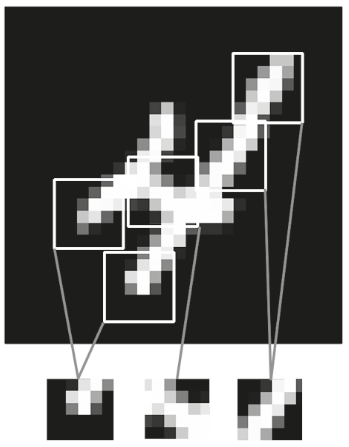
\includegraphics[width=0.4\textwidth,height=4cm,keepaspectratio=true]{content/images/LokaleMuster.png}
    \caption{Lokale Muster wie Ränder und Linien in einer handgeschriebenen Ziffer \cite[Abb. 5.1]{DeepLearningPythonKeras}}
    \label{fig:LokaleMuster}
\end{figure}

\acrshortpl{cnn} erkennen nach \cite[S. 164]{DeepLearningPythonKeras} nun diese lokalen Muster.
Chollet geht in \cite{DeepLearningPythonKeras} auf Seite 165 auf die daraus resultierenden Eigenschaften von \acrshortpl{cnn} ein.
Zunächst sei die Erkennung der lokalen Muster translationsinvariant.
Dies bedeute, dass die Muster an beliebigen Stellen im Bild erkannt werden können.
Außerdem könne durch das Hintereinanderschalten mehrer \acrshort{cnn}-Layer erreicht werden, dass Hierarchien von Mustern erlernt werden.
Aus diesen beiden Eigenschaften folgt, dass es für ein \acrshort{cnn} keinen Unterschied macht, ob die zu erkennenden globalen Muster (beispielsweise eine Ziffer) in der Eingabe verschoben sind.

Als Nächstes stellt sich die Frage, wie \acrshortpl{cnn} lokale Muster erkennen können.
Dies wird durch die Faltungsoperation erreicht.
Die Idee der Faltungsoperation ist nach \cite{6S191CNN}, einen sogenannten Filter zu verwenden, der lokale Muster erkennt.
Dieser zweidimensionale Filter wird über die 2D-Eingabe "`geschoben"' und erkennt somit, wo sich in der Eingabe ein bestimmtes Muster befindet.
Mathematisch gesehen ist ein Filter eine quadratische Matrix.
Die Elemente der Matrix sind die erlernbaren Gewichtungen, die je nach ihren Werten verschiedene Muster erkennen.
Die Erkennung geschieht dadurch, dass der Filter an der jeweiligen Stelle komponentenweise mit der Eingabe multipliziert und die einzelnen Werte anschließend aufsummiert werden.
Diese Berechnung wird in \autoref{fig:ConvExample} verdeutlicht.

\begin{figure}[h]
    \centering
    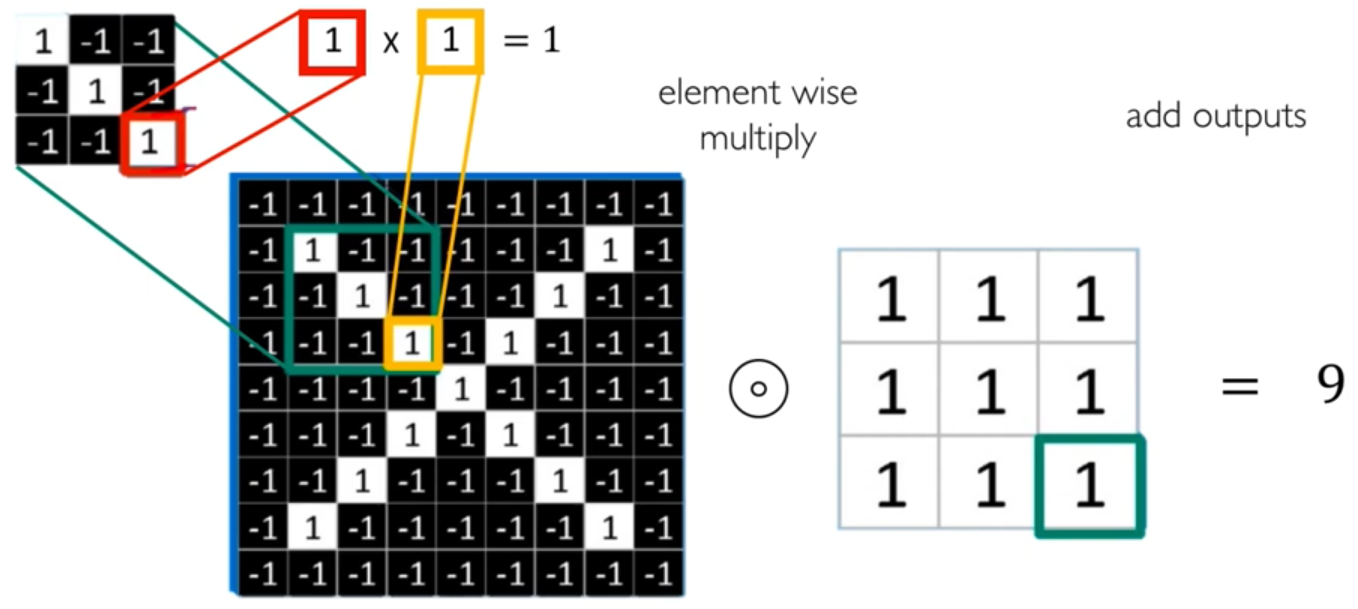
\includegraphics[width=1.0\textwidth,height=8cm,keepaspectratio=true]{content/images/ConvExample.png}
    \caption{Ein Schritt der Faltung des Filters mit der Eingabe \cite{6S191CNN}}
    \label{fig:ConvExample}
\end{figure}

Links oben in der Abbildung ist der Filter dargestellt.
Dieser Filter erkennt schräge Linien von links oben nach rechts unten.
Bei einer perfekten Übereinstimmung, wie im Beispiel der Abbildung, wird das Ergebnis der Berechnung maximal.
Angenommen, das Pixel oben in der Mitte der Eingabe wäre $1$, dann wäre das Ergebnis der Berechnung nur $7$.
Der Wert des Ergebnisses ist also ein Maß für die Übereinstimmung des Filters mit der Eingabe.
Auf dieses Ergebnis wird in der Praxis nach \cite{6S191CNN} noch eine Aktivierungsfunktion angewendet, wofür meistens \emph{\acrshort{relu}} verwendet wird.
Negative Pixel werden dadurch zu null.
Wird der Filter nun mit einer Schrittweite von $1$ in $x$- und $y$-Richtung über die gesamte Eingabe geschoben und die Berechnung jedes Mal ausgeführt, entsteht eine sogenannte Merkmalskarte (engl. \emph{feature map}).
Die Merkmalskarte gibt an, wo im Bild die Übereinstimmung mit dem durch den Filter beschriebenen Muster wie groß ist.
Damit die Merkmalskarte die gleiche Höhe und Breite wie die Eingabe hat, kann nach \cite[S. 168 f.]{DeepLearningPythonKeras} die Eingabe vor der Faltungsoperation rundherum mit Nullen aufgefüllt werden.
Dies wird auch \emph{Padding} genannt.

Nach der Faltungsoperation ist noch ein weiterer wichtiger Schritt notwendig.
Da die Merkmalskarte zunächst die gleichen Dimensionen wie die Eingabe hat, können nach \cite[S. 171]{DeepLearningPythonKeras} keine Merkmalshierarchien erkannt werden.
Das liegt daran, dass ein Pixel der Merkmalskarte nur Informationen über einen Bereich der Eingabe enthält, der so groß ist wie der Filter.
In den meisten Fällen sind dies nur 3x3 oder 5x5 Pixel.
Das Ziel ist es also, eine Merkmalskarte zu erstellen, bei der ein Pixel Informationen über einen größeren Bereich der Eingabe enthält.
Dies kann durch die MaxPooling-Operation erreicht werden, die auf die Merkmalskarte angewendet wird.
Diese funktioniert ähnlich wie die Faltungsoperation.
Auch hier gibt es einen Filter, der über die Eingabe geschoben wird.
Dieser Filter wird hier jedoch als \emph{Pool} bezeichnet.
Im Gegensatz zur Faltungsoperation wird nichts multipliziert.
Stattdessen entspricht die Ausgabe des Pools dem Maximalwert der Eingabe.
Hat der Pool beispielsweise eine Größe von 2x2 und wird in $x$- und $y$-Richtung jeweils um die Schrittweite $2$ verschoben, wird die Seitenlänge der Eingabe durch die MaxPooling-Operation halbiert.
Dies wird in \autoref{fig:MaxPooling} an einem Beispiel veranschaulicht.

\begin{figure}[h]
    \centering
    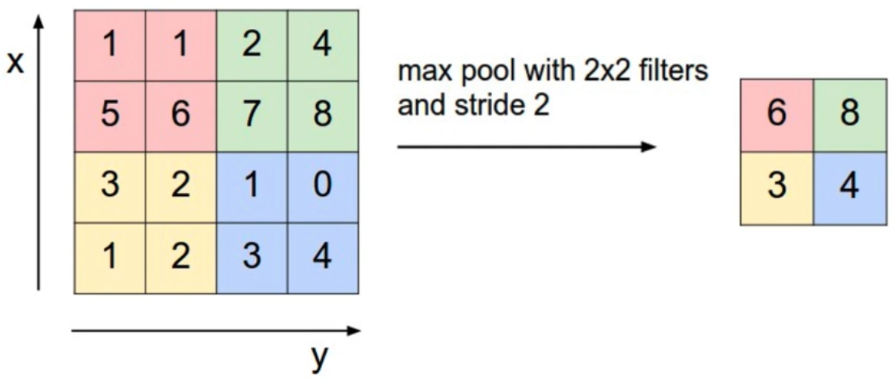
\includegraphics[width=0.8\textwidth,height=8cm,keepaspectratio=true]{content/images/MaxPooling.png}
    \caption{Beispiel einer MaxPooling-Operation \cite{6S191CNN}}
    \label{fig:MaxPooling}
\end{figure}

Werden mehrere \acrshort{cnn}- und MaxPooling-Layer abwechselnd hintereinandergeschaltet, lassen sich die Merkmale der Eingabe hierarchisch darstellen.
Dabei wird die Höhe und Breite der Eingabe nach jedem MaxPooling-Layer halbiert.
Zumm Schluss wird die Ausgabe des letzten MaxPooling-Layers an ein Feedforward-Netz zur Klassifizierung übergeben.
Das Feedforward-Netz klassifiziert die Eingabe also nun anhand von abstrakten Merkmalen, die durch die \acrshort{cnn}- und MaxPooling-Layer von \emph{beliebigen Stellen} in der Eingabe extrahiert wurden.

\subsection{Verwantete Forschung}
\label{sec:VerwanteteForschung}





\section{Verwantete Forschung}
\label{sec:VerwanteteForschung}




%%%
%%% Nachbau
%%%
\addsec{Literatur}
\renewcommand{\section}[2]{}
\bibliography{citation/quellen}
\clearpage

% Anhänge
\appendix
\addappheadtotoc
\appendixpage
\begin{appendices}
%\include{content/<Name des Anhangs>}

\end{appendices}
\end{document}
